\documentclass{beamer}
\usepackage{amsmath}
\usepackage{amssymb}
\usepackage{amsthm}
\usepackage{media9}
%\usepackage{physymb}
\usepackage{graphicx}
\usepackage{subcaption}
\iffalse
\setbeamertemplate{frametitle}
  {\begin{centering}\smallskip
   \insertframetitle\par
   \smallskip\end{centering}}
\setbeamertemplate{itemize item}{$\bullet$}
\setbeamertemplate{navigation symbols}{}
\setbeamertemplate{footline}[text line]{%
    \hfill\strut{%
        \scriptsize\sf\color{black!60}%
        \quad\insertframenumber
    }%
    \hfill
}
\fi
\newif\ifanim
\animtrue
\definecolor{DarkFern}{HTML}{407428}
\definecolor{DarkCharcoal}{HTML}{4D4944}
\colorlet{Fern}{DarkFern!85!white}
\colorlet{Charcoal}{DarkCharcoal!85!white}
\colorlet{LightCharcoal}{Charcoal!50!white}
\colorlet{AlertColor}{orange!80!black}
\colorlet{DarkRed}{red!70!black}
\colorlet{DarkBlue}{blue!70!black}
\colorlet{DarkGreen}{green!70!black}

% Use the colors:
\setbeamercolor{title}{fg=Fern}
\setbeamercolor{titlelike}{fg=Fern}
\setbeamercolor{frametitle}{fg=Fern}
\setbeamercolor{normal text}{fg=Charcoal}
\setbeamercolor{block title}{fg=black,bg=Fern!25!white}
\setbeamercolor{block body}{fg=black,bg=Fern!25!white}
\setbeamercolor{alerted text}{fg=AlertColor}
\setbeamercolor{itemize item}{fg=Charcoal}
\begin{document}
\title{Cellular Automata - An Introduction}   
\author{\begin{tabular}{r@{ }l} 
Authors:      & Manish Goregaokar, Nipun,\\ & Mohammad Qadish, Vysagh TM \\[1ex] 
Major contributors: 
             & John von Neumann\\
             & Stanislaw Ulam\\
			 & John Conway\\
             & Stephen Wolfram
\end{tabular}
\date{Date of Presentation}} 
\date{October 3, 2013} 

\frame{\titlepage} 

\part{Conway's Game of Life} \frame{\partpage}
\frame{\frametitle{The rules} 
%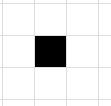
\includegraphics[scale=0.5]{images/itsaliiive.png}\\
%In the above image, a "live" cell is surrounded by eight "dead" cells
\begin{itemize}

\item {\em Loneliness\footnote{"Loneliness" is just a convenient label. Conway's Game of Life is not intended  to represent real life. However these rules can be viewed from a biological standpoint, which is one of the reasons why the automaton is called "Life"}:} A live cell with 1 or fewer neighbors dies in the next iteration
\item {\em Stasis:} A live cell with 2 or 3 neighbors lives on
\item {\em Overpopulation:} A live cell with 4 or more neighbors dies
\item {\em Reproduction:} A dead cell with exactly 3 neighbors becomes alive in the next generation
\end{itemize}
}
\frame{\frametitle{Still lifes}
\begin{center}
\renewcommand{\arraystretch}{10}\setlength{\tabcolsep}{20pt}
\begin{tabular}{cc}
 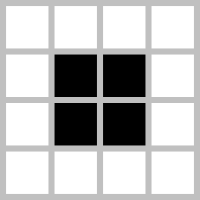
\includegraphics[scale=0.4]{images/stillblock.png} &  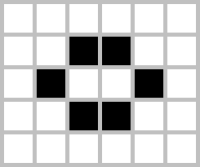
\includegraphics[scale=0.4]{images/stillhive.png}\\
  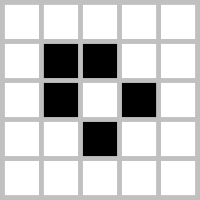
\includegraphics[scale=0.4]{images/stillboat.png} &  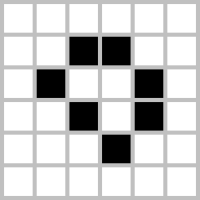
\includegraphics[scale=0.4]{images/stillloaf.png}\\
\end{tabular}
\end{center}
}

\ifanim
\frame{\frametitle{Oscillators}
\begin{center}

 \includemedia[
  activate=onclick,
 width=0.4\textwidth
]{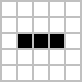
\includegraphics{images/blinkerthumb.png}}{images/Game_of_life_blinker.swf}   
\end{center}
}
\frame{\frametitle{Oscillators}
\begin{center}

\includemedia[
  activate=onclick,
 width=0.3\textwidth
]{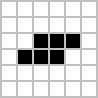
\includegraphics{images/toadthumb.png}}{images/Game_of_life_toad.swf}
\end{center}
}
\frame{\frametitle{Oscillators}
\begin{center}

\includemedia[
  activate=onclick,
 width=0.4\textwidth
]{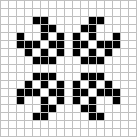
\includegraphics{images/pulsarthumb.png}}{images/Game_of_life_pulsar.swf}
\end{center}
}



\frame{\frametitle{Glider}
\begin{center}

\includemedia[
  activate=onclick,
 width=0.3\textwidth
]{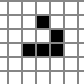
\includegraphics{images/gliderthumb2.png}}{images/Game_of_life_animated_glider.swf}
\end{center}
}
\fi

\frame{\frametitle{Motivation behind the rules}
While the biological analog seems to be a likely motivation for choosing this particular rule set, Conway's motivations are (Verbatim from the original article\footnote{Gardner, M. (1970). Mathematical Games -
The fantastic combinations of John Conway's new solitaire game "life". In {\em Scientific American} 223 (pp 120-123.)})
\begin{itemize}
\item There should be no initial pattern for which there is a simple proof that the population can grow without limit.
\item There should be initial patterns that apparently do grow without limit.
\item There should be simple initial patterns that grow and change for a considerable period of time before coming to end in three possible ways: fading away completely (from overcrowding or becoming too sparse), settling into a stable configuration that remains unchanged thereafter, or entering an oscillating phase in which they repeat an endless cycle of two or more periods.
\end{itemize}

}

\part{Generalized cellular automata} \frame{\partpage}
\frame{\frametitle{Building blocks for a cellular automaton}

To build a cellular automaton, one needs to make a suitable choice for the following:

\begin{itemize}
\item A suitable grid type. For example, we can have a 1D/2D/3D rectangular grid, a hexagonal grid, or even a Penrose tiling\footnote{Owens, N., \& Stepney, S. (2010). The Game of Life rules on Penrose tilings: still life and oscillators. In {\em Game of Life Cellular Automata} (pp. 331-378). Springer London.}
\item The number of states a cell can have. This number must be finite for it to be a cellular automaton\footnote{Otherwise it is a continuous automaton}
\item The type of neighborhood being considered. E.g. Moore, von Neumann, Margolus.
\item The rules. The rules let one calculate the next iteration of a cell given its current state and the state of its surroundings. 
\end{itemize}
}


\frame{\frametitle{Neighborhood types}
\begin{figure}
\centering
 \begin{subfigure}[b]{0.4\textwidth}
 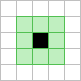
\includegraphics[scale=1]{images/Mooreneighbourhood_1cell.png}
 \caption{Moore neighborhood, range 1}
 \end{subfigure}
  \begin{subfigure}[b]{0.4\textwidth}
 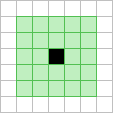
\includegraphics[scale=1]{images/Mooreneighbourhood_range2.png}
 \caption{Moore neighborhood, range 2}
 \end{subfigure} \\ ~\\~\\
  \begin{subfigure}[b]{0.4\textwidth}
 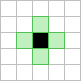
\includegraphics[scale=1]{images/Vonneumannneighbourhood_1cell.png}
 \caption{von Neumann neighborhood, range 1}
 \end{subfigure} 
  \begin{subfigure}[b]{0.4\textwidth}
 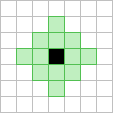
\includegraphics[scale=1]{images/Vonneumannneighbourhood_range2.png}
 \caption{von Neumann neighborhood, range 2}
 \end{subfigure} 
 % 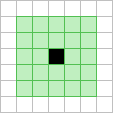
\includegraphics[scale=1]{images/Mooreneighbourhood_range2.png}\\
  %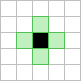
\includegraphics[scale=1]{images/Vonneumannneighbourhood_1cell.png} &  %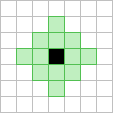
\includegraphics[scale=1]{images/Vonneumannneighbourhood_range2.png}
\end{figure}
}
\frame{\frametitle{Rules}
\begin{itemize}
\item If the evolution of a cell depends on only the sum of the states of the cell and those in its neighborhood,  the rule is {\em totalistic}.
\item If the evolution of a cell depends on only the sum of the states the cells in its neighborhood and the state of the cell itself,  the rule is {\em outer totalistic}. (E.g. Life)
\item Rules need not be totalistic
\item Rules need not be deterministic!
\end{itemize}
}

\part{Elementary cellular automata}\frame
{\partpage}
\frame{\frametitle{Rule 110}\begin{center}
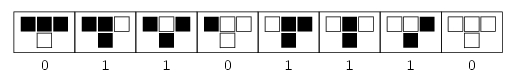
\includegraphics[scale=0.5]{images/rule110.png}\\~\\
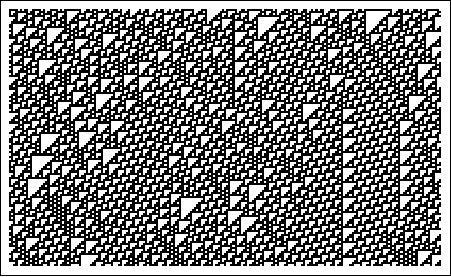
\includegraphics[scale=0.6]{images/rule110-intro.png}
\end{center}
}
\frame{\frametitle{Gliders in 110}
\begin{center}

\includegraphics[scale=0.5]{images/Ca110-structures2.png}
\end{center}
}

\frame{\frametitle{Interaction of gliders}
\begin{center}
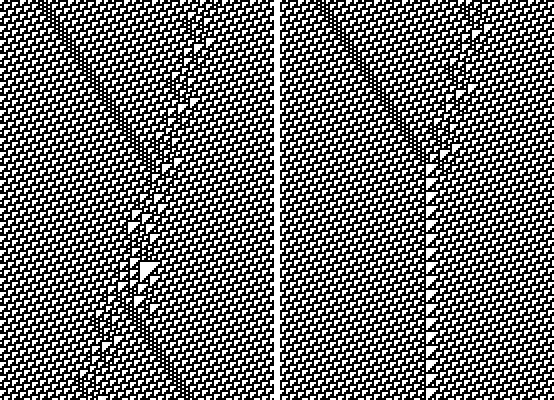
\includegraphics[scale=0.5]{images/Ca110-interaction2.png}
\end{center}
}

\frame{\frametitle{Rule 30}\begin{center}
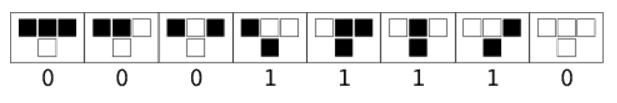
\includegraphics[scale=0.5]{images/rule30.jpg}\\~\\
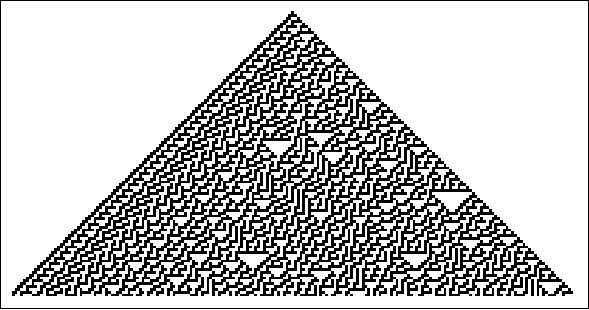
\includegraphics[scale=0.5]{images/30.png}
\end{center}
}
\frame{\frametitle{Rule 30 in nature}
\begin{center}
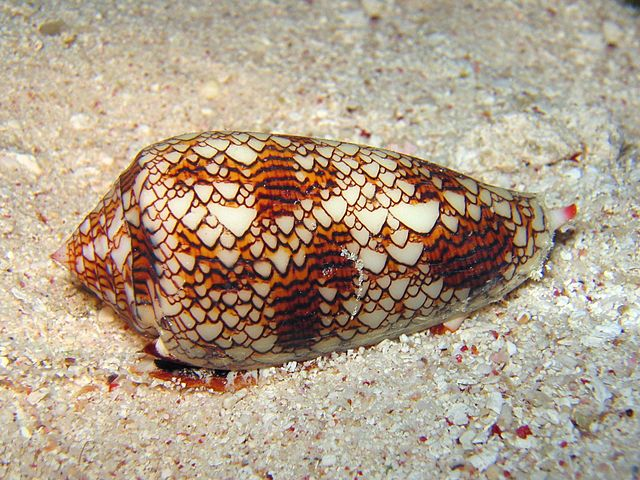
\includegraphics[scale=1]{images/640px-Textile_cone.JPG}
\end{center}

}
\part{Block Cellular automata}\frame{\partpage}
\frame{\frametitle{Margolus neighborhood}
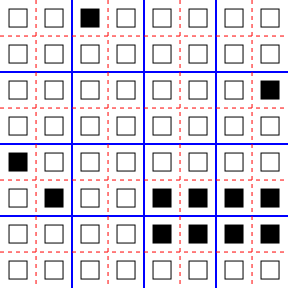
\includegraphics[scale=1]{images/Margolus.png}
}
\part{Applications}\frame{\partpage}
\frame{\frametitle{Cryptography}
\begin{itemize}
\item Pseudo-random number generators
\item Hash functions
\item Encryptions
\end{itemize}
}
\frame{\frametitle{Modelling the real world}
\begin{itemize}
\item Predator-prey interactions (stochastic)
\item Oscillatory chemical reactions
\item Lattice gases (reversible Margolus)
\item Ising model (reversible Margolus)
\item Crystal growth, shell patterns, other emergent phenomena
\end{itemize}
}
\frame{\frametitle{Miscellaneous}
\begin{itemize}
\item Universal computation in theoretical CS
\item Mental exercise; {\em Life} is one example of a CA which has been extensively researched and analyzed; with the discoveries of many new, interesting patterns. 
\end{itemize}
}
\end{document}
}
